\chapter{Tools di analisi}
In questo capitolo verranno esposti vari tools che hanno lo 
scopo di analizzare il funzionamento del DDS.
Questi tools,
a volte,
vengono anche utilizzati con altri protocolli o 
altri sistemi di rete, mentre ci sono altri tool inclusi DDSFuzz 
che sono compatibili solamente con il middleware DDS. Molti 
strumenti sono stati impiegati anche per esaminare il 
software ROS (Robotic Operation System) che utilizza come 
sistema di comunicazione un'implementazione del DDS 
(di solito Fast DDS \cite{FastDDS}) per effettuare lo scambio 
di comunicazione tra i vari dispositivi connessi.
% Mettere che wireshark e dds replay servono a fare recoinassance
%dire anche che é stato utilizzato in molti casi rti shapes

\section{WireShark}
WireShark è un tool di tipo packet-sniffing che ci consente di 
interagire e visualizzare il contenuto dei pacchetti scambiati da 
diversi protocolli di rete. Ha ottenuto un grande successo 
grazie alla sua interfaccia user-friendly e al suo codice sorgente 
open-source con licenza di utilizzo libero. I pacchetti possono 
essere analizzati sia in real-time che in modalità statica utilizzando 
un file di tipo PCAP (packet capture). 

Questo tool è anche compatibile con il protocollo RTPS che viene
adoperato dalle entità del DDS per comunicare tra di loro 
come descritto nella Sottosezione~\ref{Messages module}.
\begin{figure}[H]
    \centering
    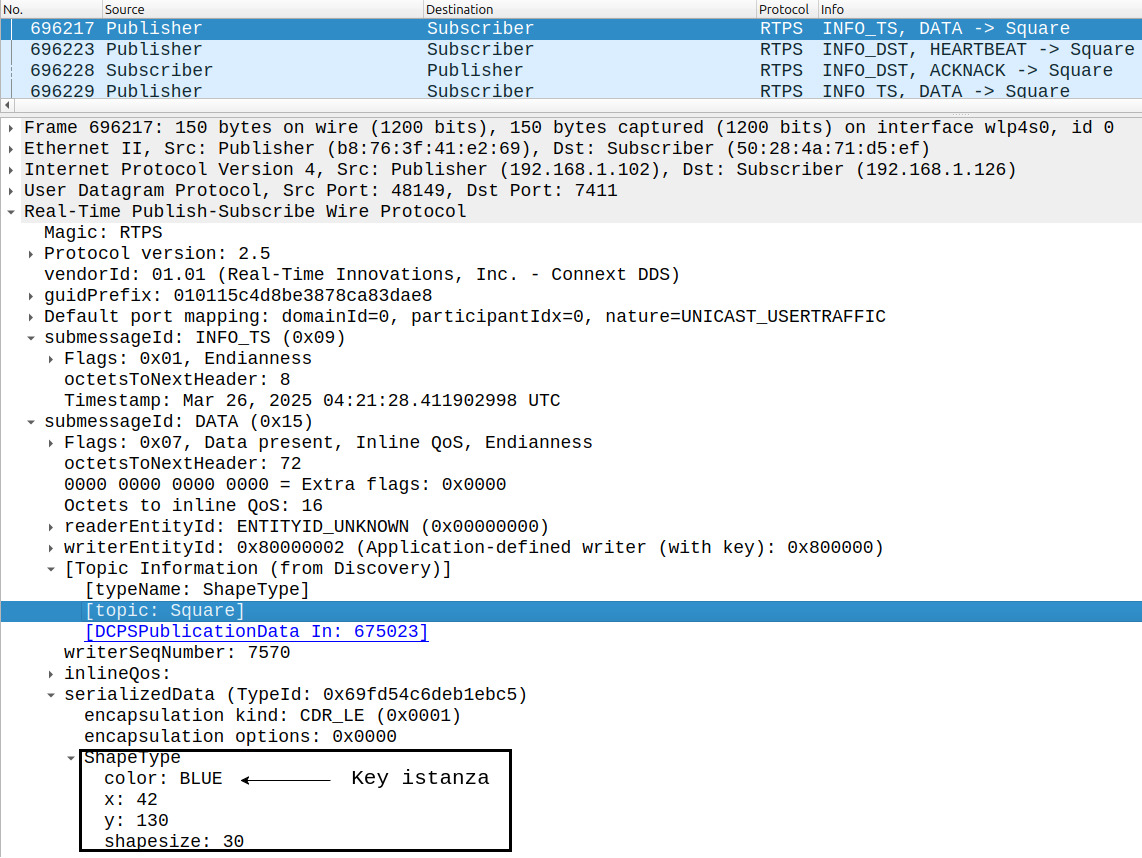
\includegraphics[width=15.2cm, keepaspectratio]{img/Info_ts e info_DST-Pagina-4.jpg}
    \caption{Esempio di cattura di un pacchetto RTPS con topic 
    Square tramite WireShark.}
    \label{wireskartshapesdemo}
\end{figure}

\subsection{Pacchetti RTPS}


\begin{figure}[H]
    \centering
    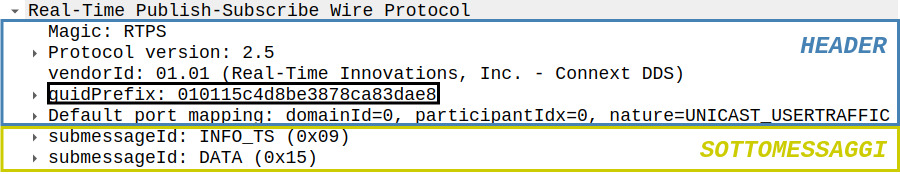
\includegraphics[width=15.2cm, keepaspectratio]{img/Header e sottomessaggi esempio shapes2.jpg}
    \caption{Pacchetto RTPS contente l'HEADER (in blu) e due sottomessaggi (in giallo).}
    \label{headersubmessagedemo}
\end{figure}



Nella Figura~\ref{headersubmessagedemo}, con l'ausilio di WireShark,
controllando il contenuto di pacchetto RTPS possiamo osservare la presenza
di un HEADER e due diversi sottomessaggi. 
\begin{itemize}
    \item All'interno dell'HEADER sono presenti
    diversi metadata, tra cui il guidPrefix, un identificativo univoco che rappresenta
    il partecipante che ha inviato il pacchetto.
    \item Il sottomessaggio INFO\_TS serve a fornire un timestamp ai destinatari 
    del pacchetto,
    quindi non contiene un guidPrefix al 
    suo interno. Al contrario, un sottomessaggio INFO\_DST include
    il guidPrefix, in quanto il messaggio è diretto a un'unica
    entità specifica, come avviene, ad esempio, per un sottomessaggio ACKNACK
    destinato a un DataWriter \cite{rtiwireshark}.
    \item Il secondo sottomessaggio, che nel nostro caso è di tipo DATA,
    serve a identificare il tipo di pacchetto.
\end{itemize}
\begin{figure}[H]
    \centering
    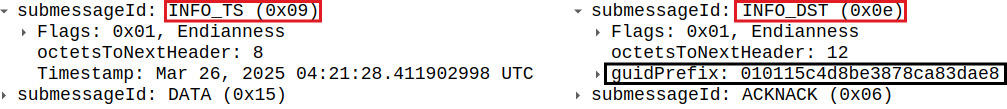
\includegraphics[width=15.2cm, keepaspectratio]{img/Info_ts e info_DST-Pagina-3.jpg}
    \caption{A sinistra sono mostrati i sottomessaggi DATA e INFO\_TS, 
    mentre a destra sono presenti i sottomessaggi ACKNACK e INFO\_DST che
    includono 
    il guidPrefix del DataWriter, lo stesso riportato in 
    Figura~\ref{headersubmessagedemo}.}
    \label{Info_ts e info_DST}
\end{figure}


\subsection{Un'alternativa a WireShark: eProsima DDS Record \& Replay}
eProsima DDS Record \& Replay è un software open-source con licenza 
Apache 2.0 sviluppato da eProsima (gli stessi creatori di Fast DDS) che 
ci consente di salvare i contenuti del traffico di un network DDS
all'interno di un file di tipo MCAP, a differenza del formato PCAP 
utilizzato da WireShark \cite{eProsimaDDSRecordeReplayDocumentation}.

MCAP è un database open-source che serve a salvare il contenuto 
di più istanze DDS (quindi provenienti da differenti flussi di dati, 
Sottosezione~\ref{Key e Istanza}), associandolo
ad un timestamp in modo tale da creare dei dati serializzati
\cite{mcap}.
Con questi dati serializzati è possibile vedere con più facilità 
il loro contenuto in modo tale da poter analizzare al meglio
il comportamento del traffico della rete, controllando nel dettaglio 
uno o più partecipanti.   

MCAP è stato creato per loggare dati provenienti da applicazioni 
che utilizzano un modello publish/subscribe, tra cui il DDS e ROS.
Quindi diversi applicativi possono interpretare questo formato, 
inclusa la piattaforma 
foxglove \cite{foxglove}, 
che consente una visualizzazione diretta dal browser e da
eProsima DDS Record \& Replay.


\section{eProsima Fast DDS Spy}
eProsima Fast DDS Spy è un tool, sviluppato da eProsima, 
open-source con licenza Apache 2.0 accessibile
tramite interfaccia a riga di comando (CLI) che serve ad monitorare i partecipanti
e i loro messaggi scambiati all'interno di una rete DDS \cite{FastDDSSpy}. 

\begin{figure}[H]
    \centering
    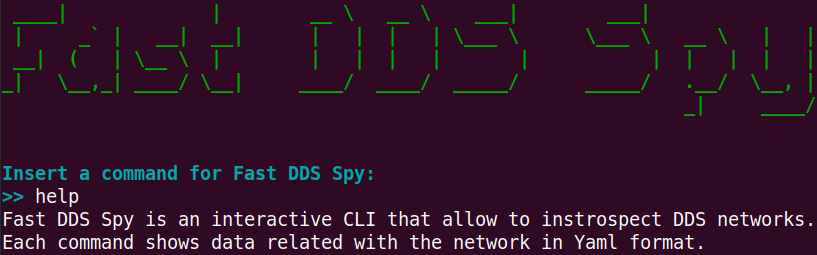
\includegraphics[width=15.2cm, keepaspectratio]{img/fastddsspyintro.png}
    \caption{Screenshot di Fast DDS Spy appena avviato.}
    \label{fastddsspyintro}
\end{figure}

Facile da utilizzare, può essere molto efficace per comprendere 
al meglio la topologia di una rete DDS. Un attaccate può usare questo 
tool per capire quali sono le varie entità del network, 
inclusi il DataWriter, il DataReader i DomainParticipant e i topic.
Per ciascuna di queste entità è anche possibile ottenere 
il loro GUID, (guidPrefix)
una stringa univoca che ci permette di identificare un partecipante.
Il GUID ottenuto può essere impiegato 
per filtrare il traffico 
real-time scambiato
all'interno della rete.

Un'altra importante funzionalità particolarmente utile per effettuare
una ricognizione del
network è offerta dai
comandi READER <GUID> e WRITER <GUID> (o in alternativa,
READER VERBOSE e WRITER VERBOSE), che mostrano
una parte delle policy QoS adoperate dai DataReader e i DataWriter.

\begin{figure}[H]
    \centering
    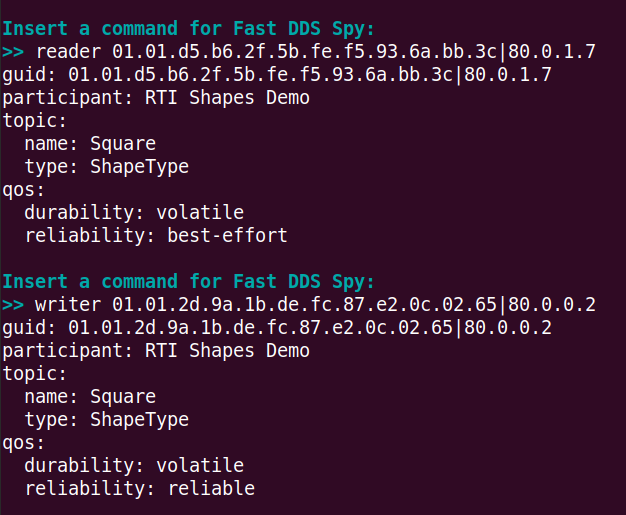
\includegraphics[width=12cm, keepaspectratio]{img/fastddsspyQoS.png}
    \caption{Esecuzione dei comandi READER <GUID> e WRITER <GUID>.}
    \label{fastddsspyQoS}
\end{figure}

\section{DDSFuzz}
DDSFuzz è un tool di analisi open source con l'obiettivo di 
effettuare test di tipo fuzz
in modo da testare vari input che il middleware DDS può
ricevere durante la sua esecuzione. Prima di questo strumento 
non esistevano (o non erano disponibili al pubblico) soluzioni
per effettuare questo tipo di test specifico sul DDS, mancanza
che DDSFuzz cerca di colmare. Infatti anche se esistono tool 
inclusi RoboFuzz e Deng, questi ultimi vengono utilizzati solamente
per testare applicativi ROS (Robotic Operation System), che 
sfruttano solo una parte delle funzioni del DDS, tralasciando
funzionalità del middleware che non vengono impegate
da ROS \cite{10.1145/3691620.3695073}.


\subsection{Fuzz testing}
Prima di parlare del tool DDSFuzz dobbiamo comprendere 
il significato di fuzzing (chiamato anche fuzz test) che è
alla base del funzionamento di questo tool. Il fuzzing è un test
automatizzato che serve a trovare e creare casi limite utilizzando
dati di input invalidi in modo tale da esplorare più vulnerabilità
possibili all'interno di un software. 
Inizialmente i primi tool di fuzzing non erano molto 
semplici da utilizzare e poco conosciuti, 
ma con il tempo questi strumenti
sono migliorati rendendoli più user-friendly e aumentando così la 
loro frequenza di uso per testare software. Oggi, il fuzzing viene
applicato a diversi tipi di applicativo, tra cui compilatori, 
applicazioni, protocolli di rete e kernel \cite{8371326}.

\begin{figure}[H]
    \centering
    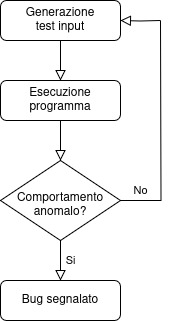
\includegraphics[width=5cm, keepaspectratio]{img/Diagramma di flusso fuzzer.jpg}
    \caption{Diagramma di flusso del funzionamento di un fuzzer.}
    \label{funzionamento fuzzer}
\end{figure}

Questi fuzzing test simulano un attacco mandando al software
che si vuole testare input regolari e irregolari, 
in modo tale da poter 
accedere ad ogni parte del codice con ogni tipo di input possibile.
In questo modo è possibile analizzare il comportamento del software
ed è possibile distinguere casi anomali o insicuri che non dovrebbero
essere possibili. Infatti quando questo test è attivo il fuzzer riceverà
varie informazioni riguardanti lo stato e l'output del programma, in 
modo tale da poter distinguere il suo comportamento. Se viene scoperto
qualche comportamento anomalo (ad esempio un segmentation fault) il 
fuzzer segnalerà in un log gli input utilizzati in modo tale da poter 
segnalare il bug.

Tuttavia, dato che questi test sono generalizzati per essere compatibili
con vari software, si crea una sorta di imprecisione nel mandare i vari 
input. Questi input a volte non sono variegati a sufficienza 
per analizzare ogni singola parte del software che stiamo analizzando.
Inoltre in molti casi può anche succedere che vengono creati
dei test che non sono necessari consumando
così risorse e tempo inutilmente.

Per migliorare la qualità di questi test è stato 
creato il DDSFuzz che essendo un fuzzer specifico solamente per 
il middleware DDS rimuove molte delle imprecisioni di un fuzzer 
più generico.

\subsection{Punti di forza del DDSFuzz}
DDSFuzz essendo specializzato per il DDS prende in considerazione 
molte sue caratteristiche che non sono presenti in altri software
o protocolli. La prima considerazione che viene 
effettuata da DDSFuzz e 
che avviene durante l'esecuzione del middleware DDS è
la topologia della rete che può mutare nel tempo creando problemi per i
fuzzer tradizionali che non si adattano ai suoi cambiamenti. Infatti certi
dispositivi si possono connettere o disconnettere dalla rete a loro 
piacimento rendendo quindi necessario cambiare i destinatari 
degli input di test 
evitando così di trasmettere informazioni verso un'entità 
che si è disconnessa e quindi impossibilitata a ricevere ulteriori
aggiornamenti. DDSFuzz prende anche in considerazione le
policy QoS e 
le funzionalità abilitate dal DDS security, come
l'autenticazione e il controllo accessi, in modo tale da
poter creare test più accurati. 

Finita l'esecuzione di DDSFuzz ci ritroviamo con due tipologie
di bug che possiamo riscontrare in un applicativo DDS:
\begin{itemize}
    \item BUG TRADIZIONALI: racchiude tutti i classici bug 
    che sono presenti anche in altri software, un esempio può 
    essere un buffer overflow;
    \item BUG SEMANTICI: questo bug avviene quando viene violata
    una norma definita dallo standard DDS,
    ad esempio un bypass dell'autenticazione. 
    Dato che il loro comportamento
    non è facilmente categorizzabile risulta più difficile individuarli;
\end{itemize}
Uno dei maggiori punti di forza di DDSFuzz sta proprio nel trovare
questi bug semantici, quasi impossibili da riconoscere per gli altri 
fuzzer. Durante l'esecuzione di DDSFuzz vengono eseguite in parallelo 
tre implementazioni (Fast DDS \cite{FastDDS}, Cyclone DDS \cite{CycloneDDS}, 
OpenDDS \cite{OpenDDS1}) vendor 
del DDS in modo tale da identificare
se i risultati dei test input rimangono consistenti tra di loro in 
ognuna delle esecuzioni. 
Se otteniamo una soluzione differente in una sola 
delle implementazioni utilizzate possiamo dire che quest'ultima ha un 
comportamento anomalo generato da un bug di tipo semantico 
\cite{10.1145/3691620.3695073}. 

\subsection{Composizione di DDSFuzz}
DDSFuzz è composto da tre elementi principali chiamati: 
DDS input generator, DDS program executor e bug detector.
\begin{itemize}
    \item DDS INPUT GENERATOR: Si occupa di generare degli input 
    specifici per il DDS prendendo in considerazione la topologia
    della rete, delle policy QoS e dei parametri di sicurezza del 
    DDS security. In questo modo non vengono generati test inutili 
    che non servono per l'analisi dell'esecuzione. 
    Questi test poi successivamente verranno adattati per essere 
    compatibili con il 
    protocollo RTPS in modo tale che il DDS program executor
    potrà utilizzarli
    immediatamente;
    \item DDS PROGRAM EXECUTOR: ricevuti gli input generati 
    li invierà alle
    tre implementazioni del DDS, mandando feedback  al DDS input generator
    sulla validità e efficacia dei test generati;
    \item BUG DETECTOR: a differenza di altri bug detector provenienti da 
    fuzzer tool generici, questo componente del DDSFuzzer riesce
    a distinguere tra bug 
    di tipo tradizionale e bug semantici, grazie all'analisi
    degli output delle implementazioni del DDS
    \cite{10.1145/3691620.3695073};
\end{itemize}